% !TeX root = ../Masterarbeit.tex
\graphicspath{{kap02/figures/}{./figures/}}
\section{A Survey on Stochastic Optimization and Chance Constraints}
\label{ch:survey}

Chapter~1 established the reliability problem and the residual-space shift. This chapter surveys the optimization paradigms and chance-constraint formulations needed to place the thesis method in context. It first distinguishes deterministic, robust, stochastic, and chance-constrained models, then reviews classical analytical reformulations and the principal sample-based and risk-based approximations. Kernel density estimation and its application literature are developed in Chapter~3, where the survey becomes the residual-space construction used by this thesis.

\subsection{Optimization paradigms under uncertainty}
\label{sec:taxonomy}

Every model under uncertainty makes two choices: what information about the random input it uses and what protection its solution provides. These choices distinguish four related paradigms.

\subsubsection{Deterministic, robust, stochastic, and chance-constrained models}
\label{ssec:paradigms}

Deterministic optimization replaces the random input by a nominal value or forecast. It is computationally attractive but does not state a probability of failure. Robust optimization instead specifies an uncertainty set $\Xi$ and requires
\begin{equation}
  g(x,\xi)\leq0\quad\text{for every }\xi\in\Xi,
  \label{eq:ch2-robust}
\end{equation}
which gives set-wise protection and may admit tractable dual reformulations~\citep{soyster1973,bental2009}. The protection depends entirely on the chosen set; a broad set can pay for physically implausible points, while an unbounded set can make the problem infeasible.

Stochastic programming consumes a probability law and optimizes expected cost. In a two-stage model, a here-and-now decision $x$ is followed by a recourse action $y(\xi)$ after the uncertainty is observed, giving an objective of the form $f(x)+\mathbb E[Q(x,\xi)]$~\citep{dantzig1955,birge2011}. This is appropriate when an adverse outcome is a cost that can be repaired. It does not, by itself, bound the frequency of an individual failure.

Chance-constrained programming uses the distribution, or samples from it, to regulate the frequency of a failure event:
\begin{equation}
  \mathbb P\{g(x,\xi)\leq0\}\geq1-\varepsilon.
  \label{eq:ch2-cc}
\end{equation}
The risk budget $\varepsilon$ is chosen by the decision maker. Chance constraints are therefore appropriate when violations are discrete events whose frequency is regulated, whereas stochastic programming is appropriate when their magnitude is priced in the objective. The paradigms are complementary formulations of the same application rather than a universal ranking. Figure~\ref{fig:taxonomy} summarizes their positions according to distributional information and protection level.

\begin{figure}[t]
  \centering
  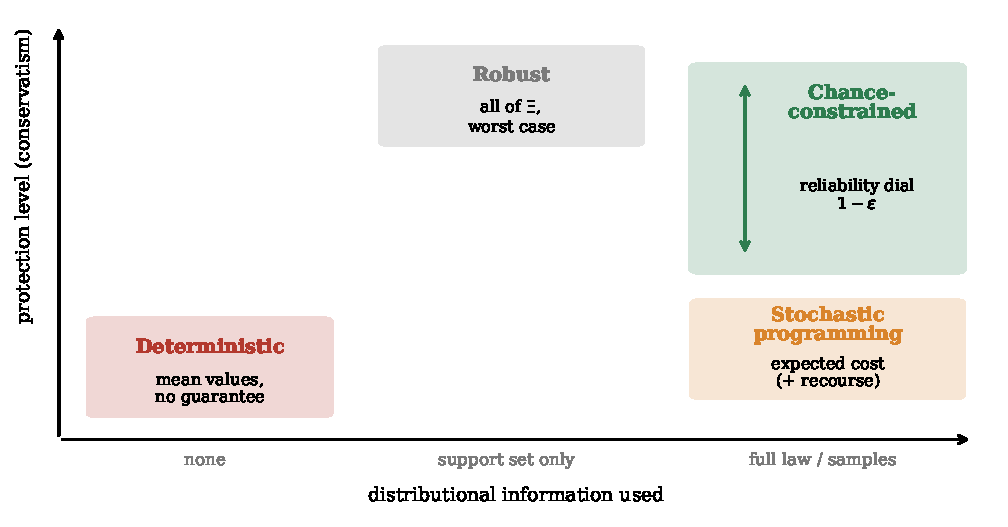
\includegraphics[width=0.85\textwidth]{fig_taxonomy.pdf}
  \caption{Four paradigms of optimization under uncertainty arranged by the distributional information used and the protection supplied. Deterministic optimization uses a point estimate; robust optimization protects a prescribed set; stochastic programming minimizes expected cost, possibly with recourse; chance-constrained programming provides a continuously chosen reliability level $1-\varepsilon$.}
  \label{fig:taxonomy}
\end{figure}

\subsubsection{Model uncertainty and distributional robustness}
\label{ssec:map}

The preceding distinction concerns what a model requires under a given law or uncertainty set. A separate question is whether the law itself is known accurately. Distributionally robust chance constraints require the probability bound to hold for every distribution in an ambiguity set. Depending on how this set is constructed, the formulation can incorporate moment information, a statistical distance from an empirical law, or another data-derived ambiguity description~\citep{calfa2015,chen2024}. The additional protection concerns uncertainty about the distribution, rather than a different definition of the failure event.

This distinction is relevant to the interpretation of KDE. Estimating a flexible density removes a fixed parametric shape restriction, but it does not eliminate estimation error or distribution shift. Throughout this chapter, a method described as nonparametric does not require a named distributional family; any reliability guarantee still depends on its sampling and regularity assumptions. The thesis studies estimators and decisions under declared sampling laws. It does not construct a distributional ambiguity set for deployment uncertainty.

\subsubsection{Individual and joint chance constraints}
\label{ssec:ch2-definitions}

Let $x\in X\subseteq\mathbb R^n$, let $\xi\in\mathbb R^d$ have law $\mathbb P$, and let $g_r$ be measurable residual functions. An individual chance constraint controls one requirement. A joint chance constraint controls all $m$ requirements simultaneously:
\begin{equation}
 \mathbb P\{g_r(x,\xi)\leq0,\ r=1,\ldots,m\}\geq1-\varepsilon.
 \label{eq:ch2-jcc}
\end{equation}
The violation form is equivalent for an individual constraint, $\mathbb P\{g(x,\xi)>0\}\leq\varepsilon$. Enforcing componentwise constraints with budgets $\varepsilon_r$ satisfying $\sum_r\varepsilon_r\leq\varepsilon$ implies~\eqref{eq:ch2-jcc} by Boole's inequality, without an independence assumption, but can be conservative when violation events overlap~\citep{prekopa1995}. The maximum residual $\max_r g_r(x,\xi)$ gives an exact scalar representation of the joint event; its non-smoothness motivates the extension in Chapter~5.

\subsection{Classical analytical reformulations}
\label{sec:classical}

\subsubsection{Canonical affine case and origins}
\label{ssec:origins}

Chance-constrained programming originated in uncertain production planning~\citep{charnes1958,charnes1959}. Early deterministic equivalents and the extension from individual to joint requirements established the basic formulation~\citep{charnes1963,miller1965}. For an affine residual
$g(x,\xi)=a(x)^\top\xi-b(x)$, the constraint is a quantile condition:
\begin{equation}
 \mathbb P\{a(x)^\top\xi\leq b(x)\}\geq\alpha,
 \qquad \alpha=1-\varepsilon,
 \label{eq:ch2-affine}
\end{equation}
with violation probability $v(x)=\mathbb P\{a(x)^\top\xi>b(x)\}$. The remaining question is whether this probability can be evaluated or reformulated without imposing an unrealistic law.

\subsubsection{Log-concavity and its boundary}
\label{ssec:logconcavity}

Pr\'ekopa's theorem identifies an important convexity island. If the law of $\xi$ is log-concave and the set $\{(x,\xi):g(x,\xi)\leq0\}$ is convex, then the satisfaction probability is log-concave in $x$; its upper level sets are consequently convex~\citep{prekopa1971,prekopa1995,prekopa2003}. Gaussian laws and uniforms on convex sets are examples. Outside these assumptions, mixtures, multimodal disturbances, heavy-tailed data, or nonlinear dynamics can destroy convexity. Figure~\ref{fig:levelsets} compares two probability level sets for the bilinear constraint $\xi^\top x\leq1$. The Gaussian panel is convex by the Gaussian second-order-cone reformulation discussed below. It is not a direct application of the jointly convex-set version of Pr\'ekopa's theorem, because the residual is bilinear in $(x,\xi)$. The mixture panel illustrates how changing the law can produce non-convex geometry with the same residual function.

\begin{figure}[t]
  \centering
  \begin{subfigure}[t]{0.48\textwidth}
    \centering
    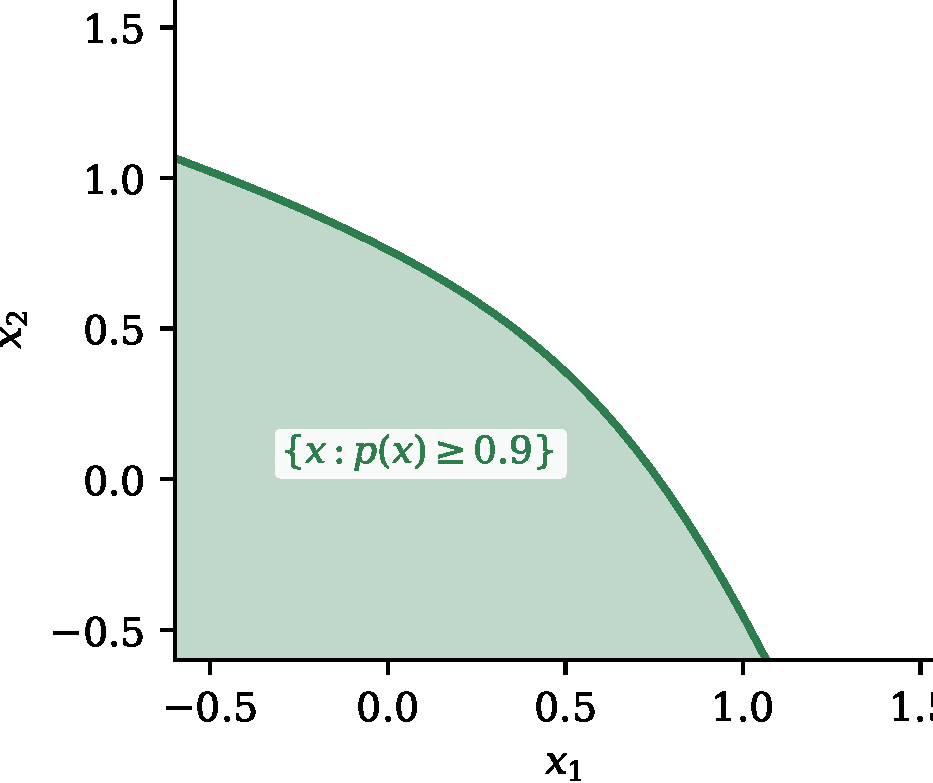
\includegraphics[width=\linewidth]{fig_levelsets_gaussian.png}
    \caption{Gaussian law: the $0.9$ probability level set is convex.}
    \label{fig:levelsets-gaussian}
  \end{subfigure}\hfill
  \begin{subfigure}[t]{0.48\textwidth}
    \centering
    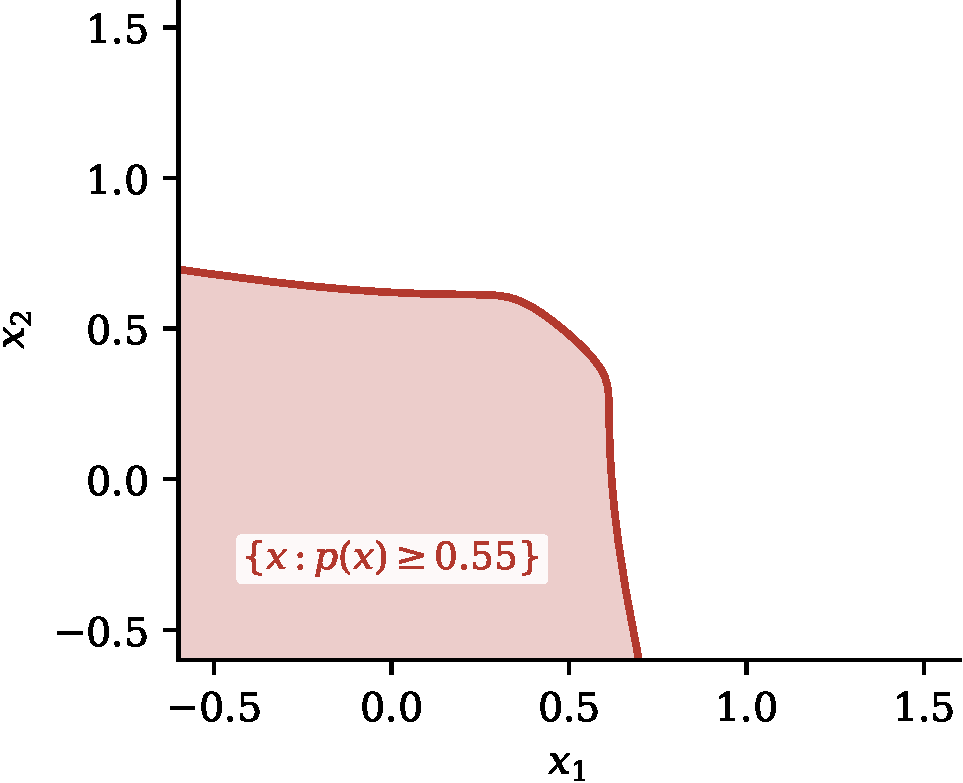
\includegraphics[width=\linewidth]{fig_levelsets_mixture.png}
    \caption{Two-component Gaussian mixture: the $0.55$ level set is non-convex.}
    \label{fig:levelsets-mixture}
  \end{subfigure}
  \caption{Convexity boundary for the computed bilinear constraint $\xi^\top x\leq1$. The Gaussian case follows the Gaussian second-order-cone representation discussed below; changing only the law to a two-component mixture produces the non-convex geometry.}
  \label{fig:levelsets}
\end{figure}

\subsubsection{General nonlinear case}
\label{ssec:generalcase}

In the general case, evaluating $v(x)$ requires integrating an unknown density over a region that changes with $x$. Even when the density is known, the region may be curved, disconnected, and high-dimensional. The approximation methods below recover tractability by conceding distributional generality, exactness, smoothness, or computational size.

\subsection{Approximation methods and their trade-offs}
\label{sec:methods}

\subsubsection{Parametric and Gaussian reformulations}
\label{ssec:gaussian}

For $\xi\sim\mathcal N(\mu,\Sigma)$ and an affine constraint, the chance constraint has the deterministic form
\begin{equation}
 b(x)-\mu^\top a(x)\geq\Phi^{-1}(1-\varepsilon)\,\|\Sigma^{1/2}a(x)\|_2.
 \label{eq:ch2-soc}
\end{equation}
When $a(x)$ and $b(x)$ are affine in $x$, $\Sigma$ is positive semidefinite, and $\varepsilon\leq1/2$, this is a convex second-order cone constraint~\citep{charnes1963,shapiro2014}. The probability reformulation is exact when the law is correct, and its conic representation is computationally efficient. The norm expression need not be differentiable at zero variance; conic solvers handle this structure directly. Its limitation is that the certificate inherits every distributional assumption: matching moments does not establish tail accuracy, and the formulation gives no internal warning when the true law is skewed, heavy-tailed, or multimodal. Spherical-radial decomposition supplies related analytic gradients for Gaussian-like laws~\citep{vanackooij2014}, but it relocates rather than removes the modeling assumption.

\subsubsection{Scenario optimization}
\label{ssec:scenario}

The scenario approach draws independent samples $\xi_1,\ldots,\xi_N$ and enforces
\begin{equation}
 g(x,\xi_i)\leq0,\qquad i=1,\ldots,N.
 \label{eq:ch2-scenario}
\end{equation}
For convex programs, scenario theory gives a distribution-free finite-sample confidence statement over IID samples from the underlying law. It does not require a parametric law, but it does require convexity and support-rank conditions. Like robust optimization, scenario enforcement protects every sampled realization; its certificate is probabilistic over the sampling process rather than a claim that the uncertainty law is absent. A standard binomial bound has the form
\begin{equation}
 \sum_{i=0}^{r-1}\binom{N}{i}\varepsilon^i(1-\varepsilon)^{N-i}\leq\beta,
 \label{eq:ch2-scenario-bound}
\end{equation}
where $r$ is an appropriate support rank and $\beta$ is the allowed confidence failure probability~\citep{calafiore2006,campi2008}. The program contains one hard constraint per sample and therefore grows with $N$; it also protects every sampled point, which can be substantially more conservative than the permitted violation budget. The guarantee does not transfer automatically to the non-convex nonlinear programs studied here.

Scenario enforcement and probability estimation should also be distinguished computationally. If each residual is smooth, each scenario constraint is smooth; the method's cost comes from the number of rows and the structure of the resulting program, rather than an indicator discontinuity. In the scalar dispatch example, enforcing every scenario gives $x_N=\max_i\xi_i$, whereas the empirical chance constraint permits a prescribed number of exceedances. This example explains possible scenario conservatism without asserting that every scenario formulation becomes more conservative in the same way or excludes sampling-and-discarding variants.

\subsubsection{Sample-Average Approximation (SAA)}
\label{ssec:saa}

SAA estimates the violation probability directly:
\begin{equation}
 \hat v_N(x)=\frac1N\sum_{i=1}^N\ind\{g(x,\xi_i)>0\}\leq\widehat\varepsilon.
 \label{eq:ch2-saa}
\end{equation}
The estimator is transparent and, under standard conditions, SAA solutions have asymptotic consistency~\citep{luedtke2008,pagnoncelli2009}. The indicator average is piecewise constant wherever no residual crosses zero, so direct differentiation gives no useful gradient between crossings. Binary variables can encode the count exactly, but this creates a mixed-integer formulation whose difficulty grows with sample size. SAA therefore trades the scenario approach's conservatism for a discontinuous or combinatorial optimization problem.

The surrogate budget $\widehat\varepsilon$ need not equal the target $\varepsilon$. A smaller budget can compensate for sampling uncertainty, provided the adjustment is justified by a statistical argument. At a fixed decision, the count is an unbiased estimate of the violation probability. At the optimizer, the same count has also influenced selection of the decision, so fixed-decision unbiasedness is insufficient to certify the selected point. Independent validation, uniform bounds over the decision class, or an applicable scenario argument address different parts of this selection problem. This distinction remains necessary when smoothing replaces the indicator.

\subsubsection{Conditional Value-at-Risk (CVaR) and convex restrictions}
\label{ssec:cvar}

For loss $L(x,\xi)=g(x,\xi)$ and confidence level $\alpha\in(0,1)$, conditional value-at-risk (CVaR) has the representation
\begin{equation}
 \operatorname{CVaR}_{\alpha}(L)=\min_{t\in\mathbb R}\left[t+\frac{1}{1-\alpha}\mathbb E(L-t)_+\right].
 \label{eq:ch2-cvar}
\end{equation}
Because CVaR dominates the corresponding value-at-risk, imposing $\operatorname{CVaR}_{1-\varepsilon}(L)\leq0$ is a sufficient, conservative restriction of the chance constraint~\citep{rockafellar2000,nemirovski2006}. Convexity is preserved when $L$ is convex in $x$ and the expectation is replaced by a sample average. The positive-part function is piecewise linear in a scalar loss. For a finite sample, auxiliary variables replace its kinks by inequality constraints that inherit the regularity of the residual map. The population expectation can also be differentiable under appropriate continuity and integrability conditions; convexity does not imply either differentiability or linearity in a nonlinear decision variable. CVaR also controls the magnitude of tail losses, so it can reject a decision with rare but large violations even when its violation frequency satisfies the chance constraint.

\subsubsection{Smooth quantiles and black-box optimization}
\label{ssec:quantile}

The chance constraint is equivalent, under the usual quantile convention, to
\begin{equation}
 Q_{1-\varepsilon}(g(x,\xi))\leq0.
 \label{eq:ch2-quantile}
\end{equation}
The empirical quantile is an order statistic and is non-smooth in $x$. Pe\~na-Ordieres, Luedtke, and W\"achter construct a differentiable sample-based quantile approximation and a trust-region SQP method~\citep{penaordieres2020}. This is a close methodological comparator because it constructs a smooth constraint from the same residual samples. Its smoothed CDF and inverse-quantile construction are closely related to integrated-kernel probability estimation. The useful distinction is which constraint representation and numerical method are used, rather than a claim that KDE uniquely provides smooth data-driven chance constraints. The present implementation evaluates the residual CDF at the fixed threshold zero; it does not benchmark the full trust-region algorithm of that paper.

A black-box method evaluates the simulator, counts failures, and optimizes using only function values, for example with pattern search or other derivative-free methods~\citep{neldermead1965,audet2017}. Its universality is useful for discontinuous or legacy simulators, but evaluations grow rapidly with decision dimension. In a discretized trajectory problem, the hundreds of decision variables make this route difficult to use as a primary method. Figure~\ref{fig:staircase} shows the underlying obstacle: the empirical violation estimate is a piecewise-constant empirical estimator, with flat regions and jumps at sampled residual crossings.

\begin{figure}[t]
  \centering
  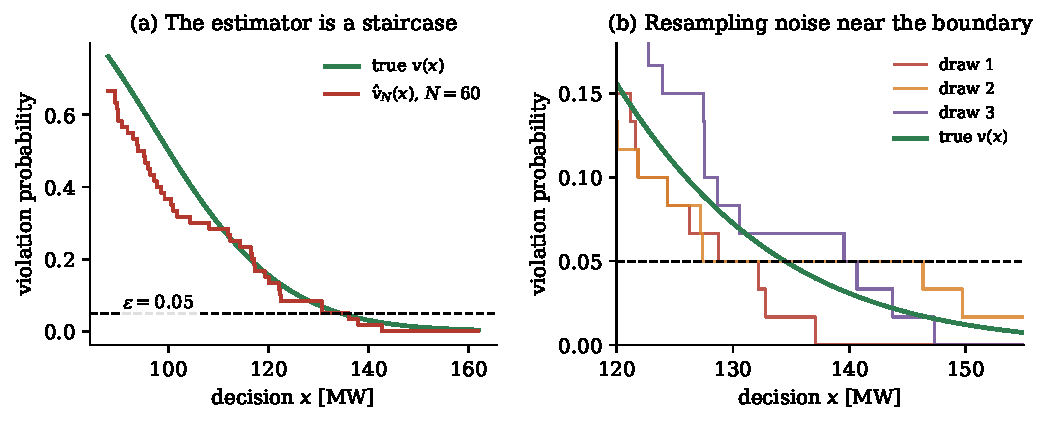
\includegraphics[width=0.82\textwidth]{fig_staircase.pdf}
  \caption{Empirical violation probability for the lognormal dispatch illustration. With $N=60$ samples the estimator is piecewise constant, and independent draws disagree near the $\varepsilon=0.05$ boundary. The figure is a seeded synthetic diagnostic of the indicator and resampling limitations.}
  \label{fig:staircase}
\end{figure}

\subsubsection{Comparison in one view}
\label{ssec:tradeoffs}

The principal alternatives partition four properties: distributional assumptions, smoothness, conservatism, and guarantee type. Here “smooth” means that the reformulated constraint supplied to the solver is differentiable; a statistical statement is not automatically a safety certificate.

\begin{table}[t]
  \centering\small
  \caption{Approximation methods for chance constraints. Guarantee labels distinguish finite-sample statements, deterministic inner bounds, statistical estimator statements, and asymptotic results.}
  \label{tab:methods}
  \resizebox{\textwidth}{!}{%
  \begin{tabular}{lllll}
    \toprule
    Method & Distribution-free & Smooth & Conservative & Guarantee\\
    \midrule
    Gaussian reformulation & No & Yes & No if correct law & Model-based\\
    Scenario approach & Yes & Yes if $g$ smooth & Often & Finite-sample$^{*}$\\
    SAA indicator & Yes & No & Tunable & Asymptotic\\
    CVaR restriction & Partial & Piecewise & Structural & Deterministic bound\\
    Smooth quantile & Yes & Yes & Tunable & Statistical\\
    Black-box DFO & Yes & No & No & None automatic\\
    Ordinary KDE & Yes & Yes & No & Asymptotic\\
    Biased KDE & Yes & Yes & By construction & Conditional\\
    \bottomrule
    \multicolumn{5}{l}{\footnotesize $^{*}$For convex programs under the assumptions of scenario theory~\citep{calafiore2006,campi2008}.}
  \end{tabular}%
  }
\end{table}

KDE is therefore not a universal winner. It is attractive when the residual map is smooth, the law is empirical or non-Gaussian, and a single smooth probability constraint is more useful than many sampled constraints. Its price is bandwidth selection, finite-sample tail error, and the need to distinguish fixed-decision envelopes from guarantees for a data-selected optimizer.
